\documentclass[../main.tex]{subfiles}
\begin{document}

\chapter{Genome-Wide Association Studies}
\labch{gwas}

\section{http://www.transplantdb.eu/sites/transplantdb.eu/files/HandsOnTutorialtoGWAS\_Seren-030715.pdf}

Genome-Wide Association Studies (GWAS) aim at identifying associations 
between genetic markers and phenotypes, \ie they find those markers that 
occur more frequently in individuals displaying a particular phenotype 
then in individuals with a different phenotype. Of course, this being a 
statistical analysis, the results have to be statistically significant; 
such reassurance, however, brings a limitation as well: since there are 
many tests of significance, multiple testing correction invalids a great 
number of results. These associations can be interpreted as the marker 
being very close to a gene controlling the phenotype under analysis, so 
close as to being in linkage disequilibrium with it; indeed, the 
association means that the marker and the allele responsible for the 
phenotype are inherited together.

Phenotypes are the product of the interaction between genotype and 
environment during development. Both contributions, the genetic one and 
the external one, are fundamental in that without any of them no living 
organism should arise (at least not one capable of \textit{evolving}). A 
GWAS focus on the genetic component as it tries to find what region of 
the genome is responsible for a given phenotypic trait. Note, however, 
that a single gene is never entirely responsible for a phenotype, for 
each gene only functions properly when it interacts with its 
environment, which includes the other genes. For instance, it would not 
make sense if there were a gene for nails without a gene for 
fingers\ldots\ Indeed, strictly speaking we cannot deem any gene as 
responsible \textit{for} any phenotype, as the phenotype depends as much 
on the gene as on the environment.

As a matter of fact, though, there are some loci in the genome which 
have a more direct influence on certain phenotypes, and these are the 
loci a GWAS is concerned with. The main purpose of a genome-wide 
association study is to find the locus which is most responsible for a 
phenotype. It is pivotal that the locus be in linkage disequilibrium 
with a genetic marker, for the marker is known and easily identifyable, 
\eg with an RFLP analysis (which is based upon gel electrophoresis), 
whereas the variant responsible for the phenotype may well be unknown or 
difficult to detect with the technologies we have at our disposal at the 
moment of the analysis. \marginnote{We should note that a typical GWA 
	study is based upon microarray data, therefore not every single 
	variant is analysed; an association study performed on 
	next-generation sequencing data is somewhat different from a GWAS.} 
Indeed, association studies can be performed to locate the approximate 
position of a genetic variant responsible for a given phenotype, in 
order to restrict the sequencing to that region so that the variant 
itself can be identified.

\section{https://onlinelibrary.wiley.com/doi/pdf/10.1002/sim.6605}

This will be useful when writing the program.

\section{https://en.wikipedia.org/wiki/Genome-wide\_association\_study}

\subsection{The structure of a GWA study}

Genome-wide association studies adopt a so-called phenotype-first 
approach, as the individuals are divided in cases and controls according 
to their phenotype only, while the genotype is accounted for only in a 
subsequent phase of the study. This can be a limiting factor for the 
analysis since, as we said above, phenotypes are the product of an 
interaction that is not biunivocal: the same phenotype can occur in 
individuals with different genotypes, and the same genotype can give 
rise to completely different phenotypes.

Another distinguishing feature of GWAS is that they investigate the 
whole genome, hence the `genome-wide' in GWAS. They are therefore devoid 
of bias due to the choice of a particular reason, and can lead to 
unexpected results.

\marginnote{As a rule, markers associated to a phenotype are not the 
	causal ones, but simply are in linkage disequilibrium with them.}

After these general considerations, we can go ahead with how a GWA study 
is performed. After having formed the two groups, namely the case group 
and the control group, containing individuals with and without the 
phenotype, respectively, the odds-ratio of each SNPs in the two groups 
is computed. If a SNP is more frequent in the case groups than in the 
control one, then its odds ratio will be greater then one. Here, the two 
odds involved in the ratio are the number of SNPs in the groups divided 
by the number of individuals in the groups. The odds ratio can be less 
than one as well, in which case it would mean that the lack of the gene 
in linkage disequilibrium with that marker is causing the phenotype, or 
that having that gene is a protecting factor against the phenotype.

Moreover, for each odds ratio a chi-squared test is performed, which 
yields a p value representing the significancy of the result. A 
Manhattan plot can thus be created, with the position on the genome on 
the X-axis, and the negative log of the p value on the Y-axis. A 
significancy threshold is set, and those markers which pass it are 
considered associated with the phenotype. Crucially, the threshold is 
chosen taking account of multiple testing issues.

\begin{marginfigure}
	\label{fig:gwas_manhattan_plot}
	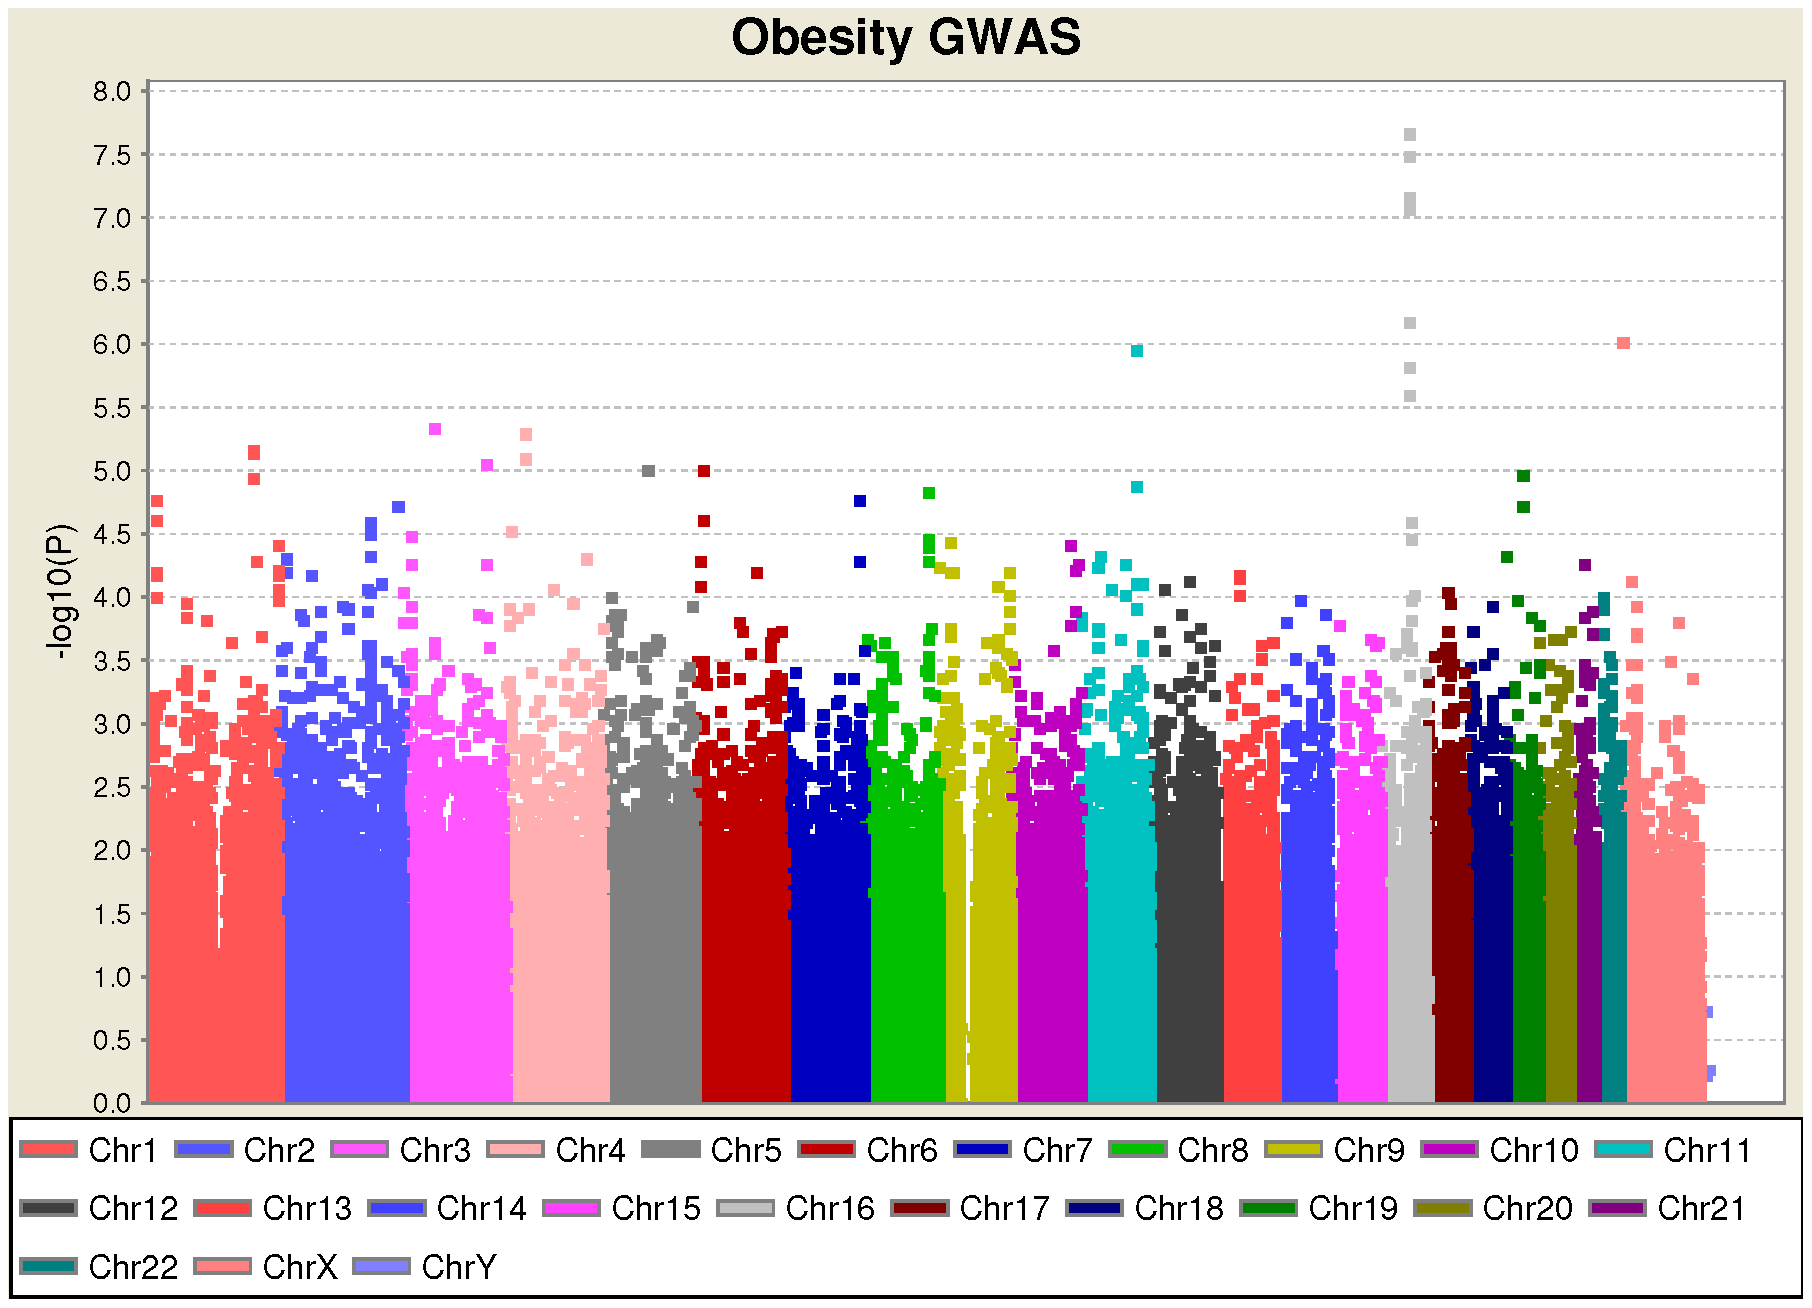
\includegraphics{gwas_manhattan_plot}
	\caption{A manhattan plot}
\end{marginfigure}

Such was the general set up of a GWA study. However, many variations are 
possible. Firs of all, should there be a distinction between homozygous 
and heterozygous individuals? I think so, but it depends on the 
phenotype: if it is due to a dominant allele, then both hetero- and 
homo-zygous individuals should count, but if the trait is recessive, 
then heterozygous individuals should be counted as not having that SNP 
at all.

Quantitative traits can be examined as well, but I think that in such a 
case a linear model would be needed instead of a simple chi-squared 
test.

Imputation is another step in many studies; briefly, it allows us to 
infer the presence of certain SNPs if others are present which are in 
strong LD with them.

Confounding factors are also taken into account to try and reduce the 
influence of the environment on the study. If we know that two 
individuals share common environmental factors -- age, for instance -- 
then the fact that they have the same phenotype is less surprising.

Finally, similar corrections can be made if the biological principles 
are considered. For instance, if protein-protein interactions are known, 
the genes coding for them could be considered as a single unit. 
\todo{The environmental factors, from the point of view of a SNP, are 
	primarily the other SNPs. Is there a way to account for that? In 
	other words, if individuals with a similar genetic background are 
	found to have the same phenotype, it is no big deal.}

\end{document}
